\documentclass{article}
\usepackage{graphicx}
\usepackage{booktabs}
\usepackage{listings}
\usepackage{xcolor}
\usepackage{hyperref}
\usepackage{caption}
\usepackage{subcaption}
\usepackage{amsmath}
\usepackage{geometry}
\geometry{a4paper, margin=1in}

\title{CS7IS2: AI Assignment 1}
\author{Rokas Paulauskas}
\date{\today}

\begin{document}

\maketitle

\begin{abstract}
    The five maze-solving algorithms—Breadth-First Search (BFS), Depth-First Search (DFS), A* Search, MDP Value Iteration, and MDP Policy Iteration are examined and their performances compared in this assignment. Such as execution time, path length, states investigated, and memory usage, are used to compare algorithms in mazes of different sizes. In addition to presenting the individual algorithm implementations, this report discusses the trade-offs among different search methods, contrasts MDP approaches, and finally compares search-based methods to MDP-based approaches.
\end{abstract}

\section{Introduction}
Maze solving is a fundamental problem in artificial intelligence and robotics. In this assignment, five different algorithms are implemented and evaluated:
\begin{itemize}
    \item \textbf{BFS} and \textbf{DFS} – classical search algorithms.
    \item \textbf{A* Search} – an informed search algorithm that uses a heuristic (Manhattan distance).
    \item \textbf{MDP Value Iteration} and \textbf{MDP Policy Iteration} – methods that address decision making under uncertainty.
\end{itemize}
The aim is to compare these methods over a range of maze sizes and analyze their performance using multiple metrics.

\section{Algorithm Implementations}

\subsection{Breadth-First Search (BFS)}
BFS explores all nodes at the current depth before moving deeper, ensuring that the shortest path is found. A snippet of the implementation is shown below.

\begin{lstlisting}[language=Python, caption=BFS Implementation]
from collections import deque

def bfs_algorithm(m):
    queue = deque([start])
    visited = set([start])
    path = {}
    explored_states = 0
    while queue:
        cur = queue.popleft()
        explored_states += 1
        if cur == destination:
            break
        for d, (dx, dy) in directions.items():
            nxt = (cur[0] + dx, cur[1] + dy)
            if nxt not in visited:
                visited.add(nxt)
                queue.append(nxt)
                path[nxt] = cur
    return path, explored_states
\end{lstlisting}

\subsection{Depth-First Search (DFS)}
DFS explores as far as possible along a branch before backtracking. It is fast but may not find the optimal path.

\begin{lstlisting}[language=Python, caption=DFS Implementation]
def dfs_algorithm(m):
    stack = deque([start])
    visited = {start}
    path = {}
    explored_states = 0
    while stack:
        cur = stack.pop()
        explored_states += 1
        if cur == destination:
            break
        for d, (dx, dy) in directions.items():
            nxt = (cur[0] + dx, cur[1] + dy)
            if nxt not in visited:
                visited.add(nxt)
                stack.append(nxt)
                path[nxt] = cur
    return path, explored_states
\end{lstlisting}

\subsection{A* Search}
A* Search combines BFS with a heuristic to efficiently guide the search towards the goal.

\begin{lstlisting}[language=Python, caption=A* Implementation]
def astar_algorithm(m):
    open_set = []
    heapq.heappush(open_set, (f_score[start], heuristic(start, goal), start))
    path, visited = {}, set()
    explored_states = 0
    while open_set:
        _, _, cur = heapq.heappop(open_set)
        explored_states += 1
        if cur == goal:
            break
        for d, (dx, dy) in directions.items():
            nxt = (cur[0] + dx, cur[1] + dy)
            if nxt not in visited:
                visited.add(nxt)
                heapq.heappush(open_set, (f_score[nxt], heuristic(nxt, goal), nxt))
                path[nxt] = cur
    return path, explored_states
\end{lstlisting}

\subsection{MDP Value Iteration}
MDP Value Iteration iteratively updates state values until convergence, then derives the optimal policy.

\begin{lstlisting}[language=Python, caption=MDP Value Iteration Implementation]
def mdp_value_iteration(m):
    explored_states = 0
    while True:
        delta = 0
        new_V = np.copy(V)
        for i in range(rows):
            for j in range(cols):
                if (i, j) == (0, 0):
                    continue
                q_vals = [rewards[next_i, next_j] + gamma * V[next_i, next_j] 
                          for next_i, next_j in neighbors]
                best_value = max(q_vals) if q_vals else V[i, j]
                new_V[i, j] = best_value
                delta = max(delta, abs(V[i, j] - best_value))
                explored_states += 1
        V = new_V
        if delta < theta:
            break
    return path, explored_states
\end{lstlisting}

\subsection{MDP Policy Iteration}
MDP Policy Iteration alternates between policy evaluation and policy improvement until convergence.

\begin{lstlisting}[language=Python, caption=MDP Policy Iteration Implementation]
def mdp_policy_iteration(m):
    explored_states = 0
    stable_policy = False
    while not stable_policy:
        while True:
            delta = 0
            new_V = np.copy(V)
            for i in range(rows):
                for j in range(cols):
                    if (i, j) == (0, 0):
                        continue
                    u = policy[i, j]
                    next_i, next_j = i + actions[u][0], j + actions[u][1]
                    if condition_met:
                        value = rewards[next_i, next_j] + gamma * V[next_i, next_j]
                    else:
                        value = V[i, j]
                    new_V[i, j] = value
                    delta = max(delta, abs(V[i, j] - value))
                    explored_states += 1
            V = new_V
            if delta < theta:
                break
        stable_policy = True
        for i in range(rows):
            for j in range(cols):
                if (i, j) == (0, 0):
                    continue
                q_vals = []
                for u, d in enumerate(directions):
                    next_i, next_j = i + actions[u][0], j + actions[u][1]
                    if condition_met:
                        q_vals.append((rewards[next_i, next_j] + gamma * V[next_i, next_j], u))
                if q_vals:
                    best_value, best_action = max(q_vals)
                    if best_action != policy[i, j]:
                        stable_policy = False
                        policy[i, j] = best_action
    return path, explored_states
\end{lstlisting}

\section{Experimental Setup}
The experiments were done on different mazes: 10×10, 20×20, 30×30, 50×50, and 100×100. For each maze, the following were measured:
\begin{itemize}
    \item \textbf{Execution Time (s)}: Total time taken to find solution.
    \item \textbf{Path Length}: Number of steps for solution.
    \item \textbf{States Explored}: How many steps were checked for solution.
    \item \textbf{Memory Usage (KB)}: Memory consumption during execution.
\end{itemize}
The maze was generated with a 40\% loop percentage to ensure sufficient complexity while maintaining feasibility in execution time.

\section{Results and Analysis}
Figures below show the performance trends for each algorithm over different maze sizes.

\subsection{Execution Time}
\begin{figure}[h]
    \centering
    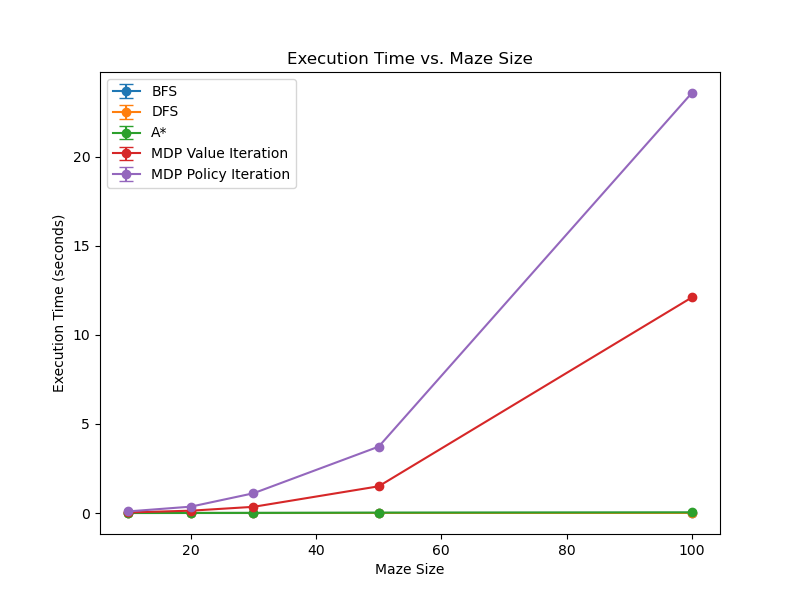
\includegraphics[width=0.8\textwidth]{analysis_plots/execution_time.png}
    \caption{Execution Time vs Maze Size}
\end{figure}

\subsection{Path Length}
\begin{figure}[h]
    \centering
    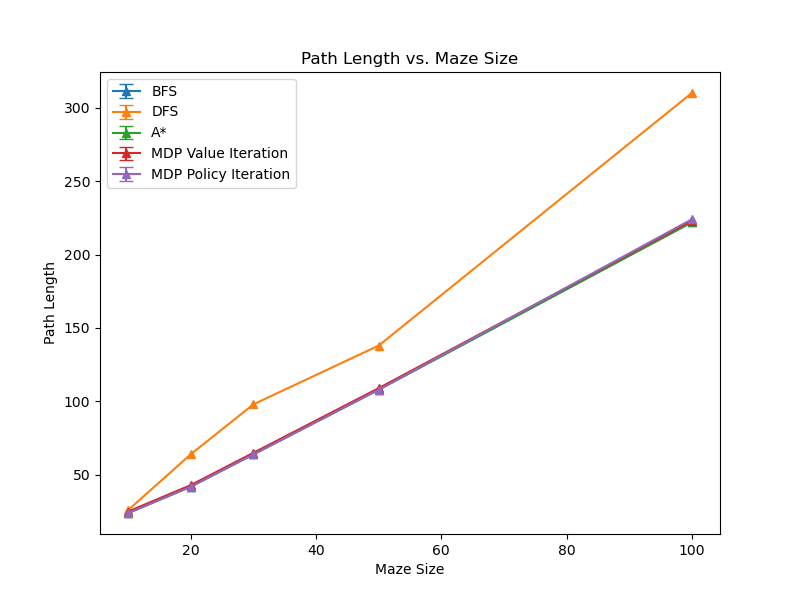
\includegraphics[width=0.8\textwidth]{analysis_plots/path_length.png}
    \caption{Path Length vs Maze Size}
\end{figure}

\subsection{States Explored}
\begin{figure}[h]
    \centering
    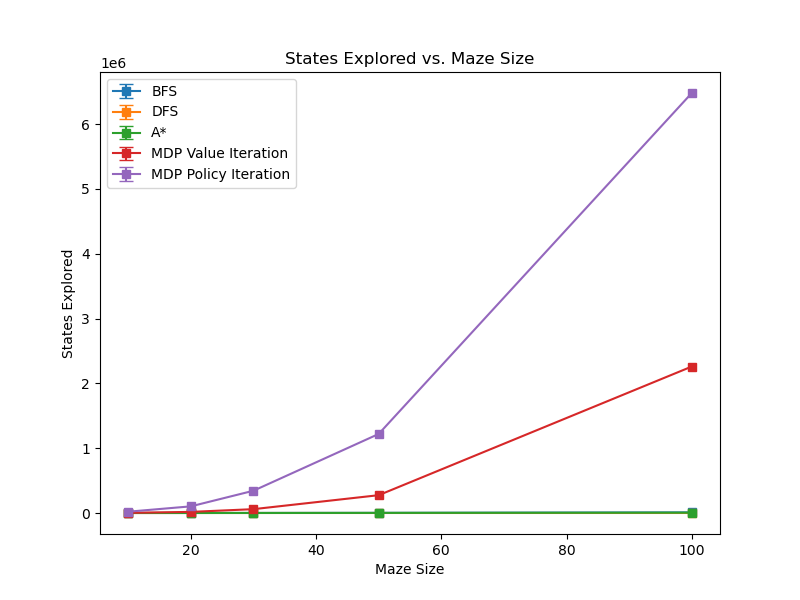
\includegraphics[width=0.8\textwidth]{analysis_plots/states_explored.png}
    \caption{States Explored vs Maze Size}
\end{figure}

\subsection{Summary Statistics}
Table \ref{tab:summary_statistics} shows the aggregated performance metrics.

\begin{table}[h]
    \centering
    \caption{Summary Statistics of Algorithm Performance}
    \label{tab:summary_statistics}
    \begin{tabular}{lcccccc}
    \toprule
    Algorithm & Time (s) Mean & Time (s) Std & States Explored Mean & States Explored Std & Path Length Mean & Path Length Std \\
    \midrule
    A*                     & 0.0125  & 0.0173  & 1608.2   & 2573.3   & 94.4   & 86.4   \\
    BFS                    & 0.0039  & 0.0060  & 2776.8   & 4141.7   & 94.4   & 86.4   \\
    DFS                    & 0.0016  & 0.0012  & 217.8    & 198.3    & 134.4  & 128.8  \\
    MDP Policy Iteration   & 5.6615  & 9.7971  & 1647088.0& 2769879.1& 94.4   & 86.4   \\
    MDP Value Iteration    & 2.7214  & 4.9994  & 525545.2 & 976236.2 & 95.4   & 86.4   \\
    \bottomrule
    \end{tabular}
\end{table}

\section{Comparative Analysis}

\subsection{Search Algorithms (BFS, DFS, A*)}
Among the search algorithms:
\begin{itemize}
    \item \textbf{BFS} guarantees the shortest path but explores many states.
    \item \textbf{DFS} is the fastest in terms of execution time but often results in suboptimal paths.
    \item \textbf{A*} offers a good balance between exploration and optimality due to the use of a heuristic.
\end{itemize}
The experimental results indicate that while DFS is fastest, its path quality suffers compared to BFS and A*.

\subsection{MDP Algorithms (Value vs Policy Iteration)}
The two MDP methods differ significantly:
\begin{itemize}
    \item \textbf{MDP Value Iteration} converges faster in some cases, but its performance is sensitive to the chosen parameters (e.g., gamma, theta).
    \item \textbf{MDP Policy Iteration} generally achieves a stable policy, albeit with a higher computational cost.
\end{itemize}
Both methods are computationally more expensive compared to search algorithms, but they provide a robust framework in uncertain environments.

\subsection{Search vs MDP Algorithms}
When comparing search-based methods to MDP-based methods:
\begin{itemize}
    \item \textbf{Search Algorithms} are more efficient in deterministic maze environments.
    \item \textbf{MDP Methods} have advantage in scenarios where the environment has uncertainty or varying rewards, despite their higher computational demands.
\end{itemize}
The advantages and disadvantages have to be chosen between execution time and robustness.

\section{Discussion and Design Choices}
Key design choices include:
\begin{itemize}
    \item \textbf{Heuristic for A*}: The Manhattan distance was chosen for its simplicity and effectiveness in grid-based mazes.
    \item \textbf{MDP Parameters}: The values of gamma and theta were selected based on preliminary experiments to balance convergence speed and solution quality.
    \item \textbf{Maze Generator}: A loop percentage of 40\% was used to ensure a reasonable challenge without making the maze unsolvable.
\end{itemize}
These choices are confirmed by the experimental outcomes, which show clear performance trends that align with theoretical expectations.

\section{Conclusion}
This report has presented an in-depth analysis of five maze solving algorithms. While search algorithms (BFS, DFS, A*, etc.) are well-suited for deterministic settings, MDP methods offer a viable alternative when dealing with uncertain or dynamic environments. The comprehensive performance analysis using multiple metrics demonstrates the trade-offs between execution speed, optimality, and computational resources.

\section*{Appendices}
\subsection*{Appendix A: BFS Implementation}
\lstinputlisting[language=Python]{bfs.py}

\subsection*{Appendix B: DFS Implementation}
\lstinputlisting[language=Python]{dfs.py}

\subsection*{Appendix C: A* Implementation}
\lstinputlisting[language=Python]{astar.py}

\subsection*{Appendix D: MDP Value Iteration Implementation}
\lstinputlisting[language=Python]{MDP_value.py}

\subsection*{Appendix E: MDP Policy Iteration Implementation}
\lstinputlisting[language=Python]{MDP_policy.py}

\end{document}
